\chapter[Physical Geography]{The Korean Peninsula: Physical Geography, Water and Climate Change}
\chapterauthor{Marc Los Huertos}

\section{Framing the Peninsula's Physical Geography}

The Korean Peninsula endenders a wide range of geographic characteristics that potential environmental risks. For our purposes, I have tried to frame the environmental issues of the peninsula within the following questions: 

\begin{enumerate}
  \item What are the defining features of the geo-physical context of the Korean Peninsula? 
 
  \item What challenges do they pose to the analysis of environmental issues? 
\end{enumerate}

In particular, I will summarize the geologic context, describe the climate and water resources and put them into context of climate change and water use, and energy use scenarios. 

Since Korea has no source of oil, what are the energy issues; what are the water issues...and how do these impact food security?


%4.	There are few areas that might not be necessary, like Korean Diet and Westernizing diet (page 13-14)

%I can go over more details with you after class tomorrow around 4. We can look at my corrections together. Don�t worry about not having time to include all of the changes. We are planning to revise the essays after the conference for the edited volume. 




\section{Geologic Context}

\subsection{North China Craton}

The Korean terrain is the result of some 3.85 billion years of geologic processes. In particular, tectonic forces and processes. On a superficial basis the the Korean peninusula part of Asian continent -- but the continent is not made up on one homongenous piece of the Earth's crust, but is composed of a set of cratonic blocks and each one has their own history and development (Figure~\ref{fig:EastAsia}). The Korean Peninsula lies on the North China Craton, one of the oldest fragments of a continent with rocks over 3.85 billion years old

%(Figure~\ref{liu1992remnants}). 

\begin{figure}[h!]
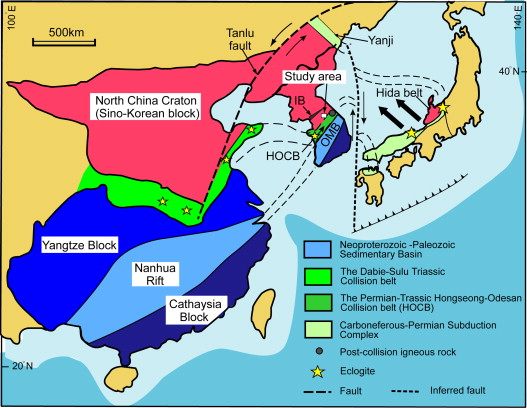
\includegraphics[width=\textwidth]{EastAsiaTectonics}
\label{fig:EastAsia}
\end{figure} 

Even the deep history of the NCC is one subjected to a wide range of tectonic activity. At a large scale the block appears homogenous, in part because systematic research began in the early 21st century. Since the 2000s, the complexity of the craton is being better appreciated --- in terms of its origin and how it has evolved over time \citep{zhao2005late}. 

Specifically, the North Korean portion of the peninsula shares some of this early history (Figure \ref{fig:NCC_history}).

\begin{figure}[h!]
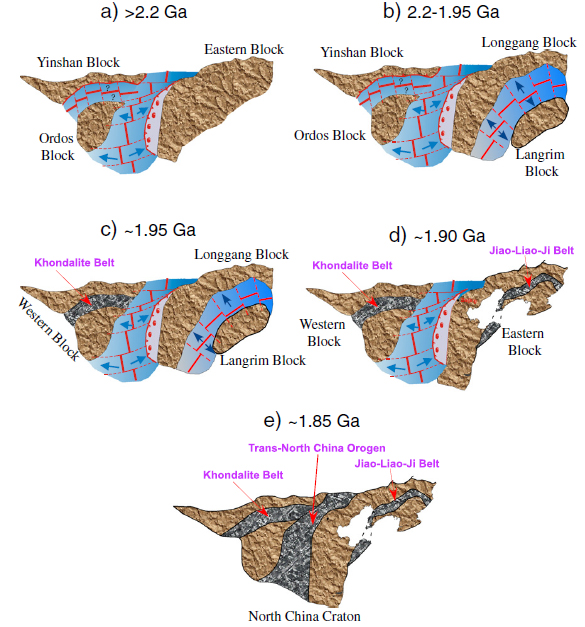
\includegraphics[width=\textwidth]{Zhao_2013_Lithotectonic}
\caption{Hypothesized early geologic history of the North China Craton \ref{zhao2013lithotectonic}.}
\label{fig:NCC_history}.
\end{figure}

And as a continent, East Asia is composed in part from several cratons, the North China Craton, South China Craton and Tarim Craton. The amalgamation of these cratons did not occur until early Cretaceous and Tertiary (Figure~\ref{fig:NCC}).

\begin{figure}[h!]
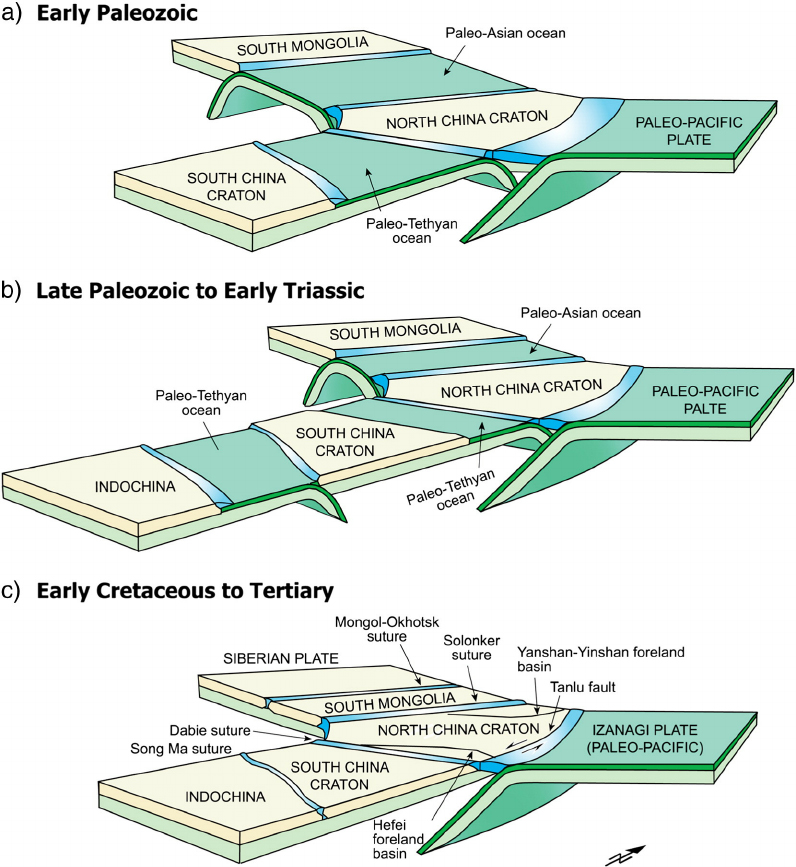
\includegraphics[width=\textwidth]{NCC_Collisions}
\caption{ (Source: \citet{kusky2014flat}.}
\label{fig:NCC}
\end{figure}

\subsection{Korean Peninsula Geology}

In spite our delayed understanding of the NCC complexity, geology of the Korean Peninsula is documented before the Second World War (Figure~\ref{fig:kobayashi}). 

\begin{figure}[h!]
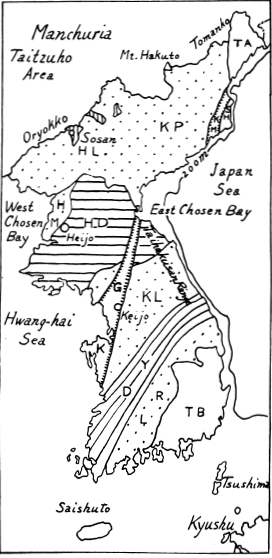
\includegraphics{Kobayashi_1933}
\caption{ (Source: \citet{kobayashi1933sketch}). }
\label{fig:kobayashi}
\end{figure}


\citet{ree1996possible}


Finally, we begin to appreciate the complexity of the Peninsula with a recently published review for the Olympics (Figure~\ref{fig:olympics}).

\begin{figure}
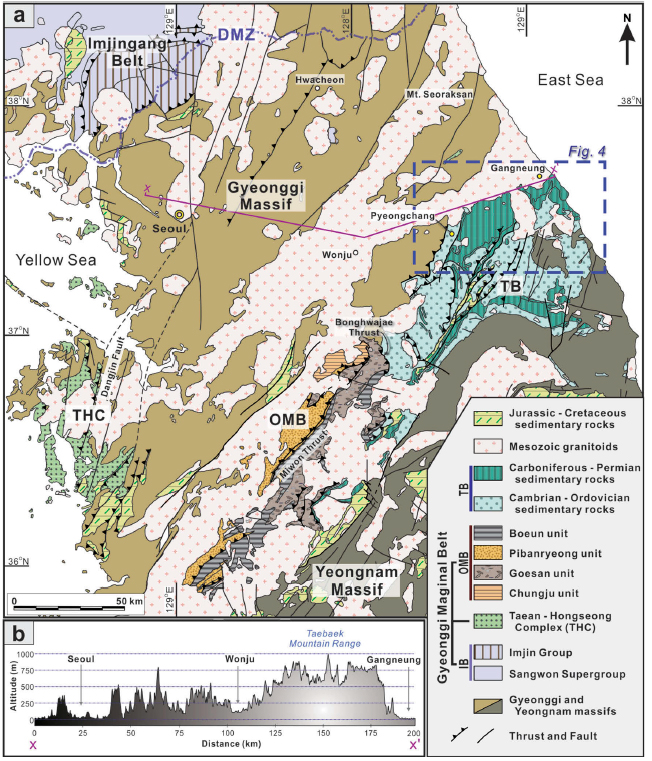
\includegraphics[width=\textwidth]{Cho_winter_olympics}
\caption{ (Source: \citet{cho2018geology}).}
\label{fig:olympics}
\end{figure}

\section{Aquascape: Climate and Water Demand}

The peninsula's water landscape relies on precipation and it's storage -- behind dams and in aquifers. 

(Figure~\ref{fig:groundwater}).

\begin{figure}
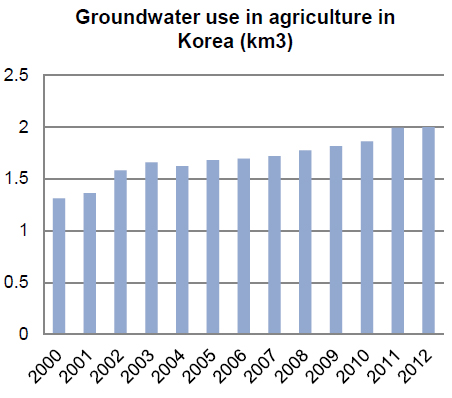
\includegraphics[width=\textwidth]{Groundwater}
\caption{ Source:\citet{TBD}.)}
\label{fig:groundwater}
\end{figure}

\citep{lee2007hydrological}


\subsection{A Shared Future on a Divided Peninsula}

The Korean Peninsula has been subjected to constant barrage of colonial projects from the North, West and East. Since the Korean Conflict, the Peninsula's ecology has been subjected to a geopolitical concerns resulting divergent and convergent socio-economic and environmental outcomes. And yet, the political boundaries have artificially cut the Imji and Bukhan river watersheds; the forests species are shared; and the Peninsula will experience similar climate change trends.  

While both countries import food. their food systems can be thought of different manifestations of similar issues and and with solutions that might be ``shared.'' In 2006, the World Food Program (WFP) and FAO estimated a requirement of 5.3 to 6.5 million tons of grain when domestic production fulfilled only 3.825 million tons. The country also faces land degradation after forests stripped for agriculture resulted in soil erosion. Harsh weather conditions that dented the agricultural output (wheat and barley production dropped 50\% and 80\% respectively in 2011) and rising global food prices stressed greater food shortage, putting 6 million North Koreans at risk.

The yield in food production in 2016 increased by 7 percent from 4.5 million tonnes in 2015 to 4.81 million tonnes and North has produced more food than South. It is estimated production decreased by 2\% in 2017 to 4.71 million tonnes.

As an industrialized, lower populated portion the North's economic development was considerably higher until the 1970s when the higher populated and largely agricultural base industrialized and showed rapid growth, along with the other Asian tigers during that time. In recent times the S. Koreans are known for heavy industry, electronics, and XX. Meanwhile with the collapse of the Soviet Union and economic sanctions and trade-embargoes the north's development has been severely constrained. The aggravated chronic food shortages of the 1990's has been continued by on-going systemic problems including a lack of arable land, collective farming practices, and persistent shortages of tractors and fuel. 

These histories have dramatic impact on the natural resources and food production in the countries...

In the south, arable land reached a maximum in 1968 (2.31 m ha) while trying to meet food requirements, but with economic success, the reliance on food aid ended in the late 1960s and the ROK began food demand for meats increased and over time in-country production was focused on staples (e.g. rice, which the country was self-sufficient in 1978) and imports meats and dairy. 

\subsection{Climate Trends}

\subsubsection{Data Sources}

Climate data was obtained climate data from the National Oceanic and Atmospheric Administration, Climate Data Online and access in January 2018 (\url{www.ncdc.noaa.gov}). R, an open source programming environment \citep{CRAN}, was used to analyze and display the data and the SPIGA package to analyze the standardize drought index \citep{SPIGA}, based on \citet{belayneh2012standard}.

\subsection{Temperature}

\subsubsection{Maximum Temperatures}

The daily maximum temperature records generally being in the mid-20th century and demonstrate an increasing trend. These trends vary between stations and are often limited to a few months a year. Most of the stations have increasing trends in March, June and September show an statistically significant trend, while Illeungdo Island is significant from Jan - June, but nothing later in the year. Finally, Makpo was significant from Jan - May, but not afterwards. These data suggest maximum daily temperatures are increasing in a pronounced way in Korea first half of the calendar year. 

\begin{figure}[h]
\label{fig:temppyongyang}
\caption{Max Temp. Pyongyang}
\includegraphics[width=\textwidth]{"TMAX_PYONGYANG INTERNATIONAL, KN"}
\end{figure}

In sum, based on the evaluation of four sites, the number of months with significant trends range from 3 to 8 (Table~\ref{tab:tmax}).

\begin{table}[h]
\caption{Trends in TMAX}
\label{tab:tmax}
\begin{tabular}{llp{4cm}}\hline
Station     &   Temperature Rate Range    & No. of Months with Warming (p < 0.05) \\ \hline\hline
Incheon (ROK) & 0--.04\degree/yr      & 8 \\
Mokpo   (ROK) & -0.01--0.02\degree/yr      & 5 \\
Pyongyan (DPRK) & 0--0.04\degree/yr      & 3 \\
Ulleungdo (ROK) & -0.01--0.03\degree/yr      & 3 \\
\hline
\end{tabular}
\end{table}


\subsubsection{Minimum Temperatures}

More important, are the increasing minimum temperatures, for example, in Icheon, 7 months has a significant increase monthly min daily temperatures and Pyongyang has a significant trend 10 out of 12 months (Figure~\ref{fig:mintemppyongyang}).

\begin{figure}[h]
\label{fig:mintemppyongyang}
\caption{Min Temp. Pyongyang}
\includegraphics[width=\textwidth]{"TMIN_PYONGYANG INTERNATIONAL, KN"}
\end{figure}

In sum, based on the evaluation of four sites, the number of months with significant trends range from 2 to 10 (Table~\ref{tab:tmin}).

\begin{table}[h]
\caption{Trends in TMIN}
\label{tab:tmin}
\begin{tabular}{lp{4cm}p{4cm}}\hline
Station     &   Temperature Rate Range    & No. of Months with Warming (p<0.05) \\ \hline\hline
Incheon (ROK) & 0.01-0.03\degree/yr      & 7 \\
Mokpo   (ROK) & 0-0.01\degree/yr      & 2 \\
Pyongyan (DPRK) & 0.02-0.07\degree/yr      & 10 \\
Ulleungdo (ROK) & 0-0.03\degree/yr      & 5 \\
\hline
\end{tabular}
\end{table}


\subsection{Precipitation}

\subsubsection{Rainfall}

Precipitation trends are harder to summarize because in some cases, the rainfall trend is upward in others it's downward, depending on the month and station selected. Rainfall on the Peninsula seems to be responding is several uneven ways, increasing monthly totals and decreasing depending on the station and the month. 

trends have so much noise it is difficult to determine if there are valid observations to generate a policy response (Table~\ref{tab:pcrp}). However, \citet{bae2008long} found declining rainfall in April in the south-western portion of the Peninsula relying on approximately 300 high quality weather stations. Because the available records via NOAA are relatively scant, it's no surprise that the results do not agree and in fact, the variable responses suggest that a signal cannot be found using these data. Furthermore, the stations analyzed do not cover the south-west corner and found insignificant results for the Han, Nakdong, and Gum river watersheds. 

\begin{table}
\caption{Trends in PRCP}
\label{tab:prcp}
\begin{tabular}{llll}\hline
Station     &   Increasing Months (NS)    & Decreasing Months (NS)  & No Sig Change \\ \hline\hline
Incheon (ROK) & none (5)    & none (4)    & 12 months  \\
Mokpo   (ROK) & none (6)    & none (6)    & 12 months   \\
Pyongyan (DPRK) & May (7)   & none (5)   & 11 months \\
Ulleungdo (ROK) & May, Aug (3) & 5 Jan (6)  & 9 months \\
\hline
\end{tabular}
\end{table}

Rainfall and temperature, of course, interact on the landscape and reference evapotranspiration (ET$_o$) is a key indicator of that impact on water resources because as an index is signals water demand by plants with implications for forests and crop production. 

In a study by \citet{nam2015has}, the mid- and southwest have experienced in increase in ET$_o$ during the months of February, March, and November since the 1970s. These results have important implications to manage water resources, since ground water may be the only source to counteract an increase in ET$_o$.

\subsubsection{Snow Depth}

Precipitation as snow is one of the most important forms of precipitation for many countries because snow provides water storage, slow discharge rates that are easier to capture, and improves soil infiltration and ground water recharge. However, the records of snow depth collected by weather stations is inadequate to quantify long-term trends because their locations have such limited recorded snow events.

IS THERE ANOTHER SOURCE? So far, can't find.

\subsection{Extreme Events}

Drought and flooding have had differential impacts on the Peninsula. The floods in North Korea in 1995 were devastating -- generating landslides, destroying crops, and causing loss of live.

The long-term weather changes have been have not be obvious. In fact, Korea experienced a dramatic drought between 2013-2015. Although the drought was only three years, it exposed concern that the Peninsula could continue to experience drought even while an increase in precipitation trends exists. However, the history of drought longevity and severity suggest that this recent event was mild compared to previous events (Figure~\ref{fig:korea_droughts}). 

\begin{figure}[h]
  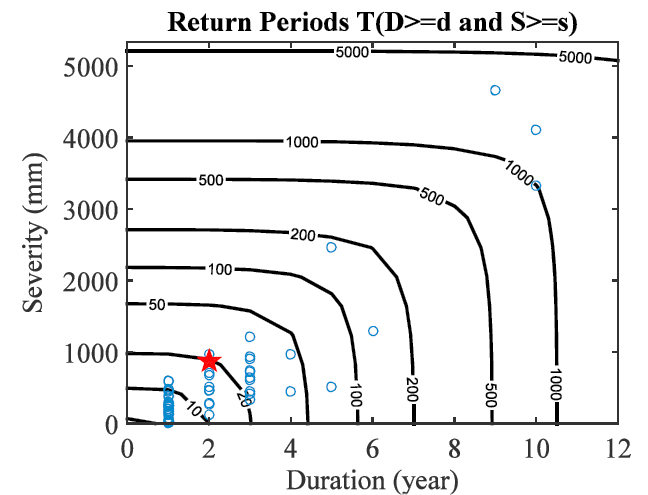
\includegraphics[width=\textwidth]{korea_drought_returninterval}
  \label{fig:korea_droughts}
  \caption{Severity and Longevity of drought in Korea (Source: \citet{kwon2016unusual}). Red star corresponds to the 2013-15 drought.}
\end{figure}

In fact, using data for Pyongpang, there does not appear to be a long-term trend of increasing or decreasing precipitation totals (Figure~\ref{fig:drought}).
\begin{figure}[h]
\caption{Standardized Precipitation Index for Pyongpang (1939-2018).}
\label{fig:drought}
\includegraphics[width=\textwidth]{"SPIGA_3MonthlyPRCPSum"}
\end{figure}

\subsection{Climate Scenarios and Natural Resources}

\subsubsection{Storage -- Groundwater and Surface Water}

Although data from N Korea are scant, ROK uses a significant portion of groundwater for both drinking and irrigation (Figure~\ref{fig:ROK_groundwater}).

\begin{figure}[h]
\caption{Proportion and Use of Groundwater in ROK (Source: \citet{TBD}).}
\label{fig:ROK_groundwater}
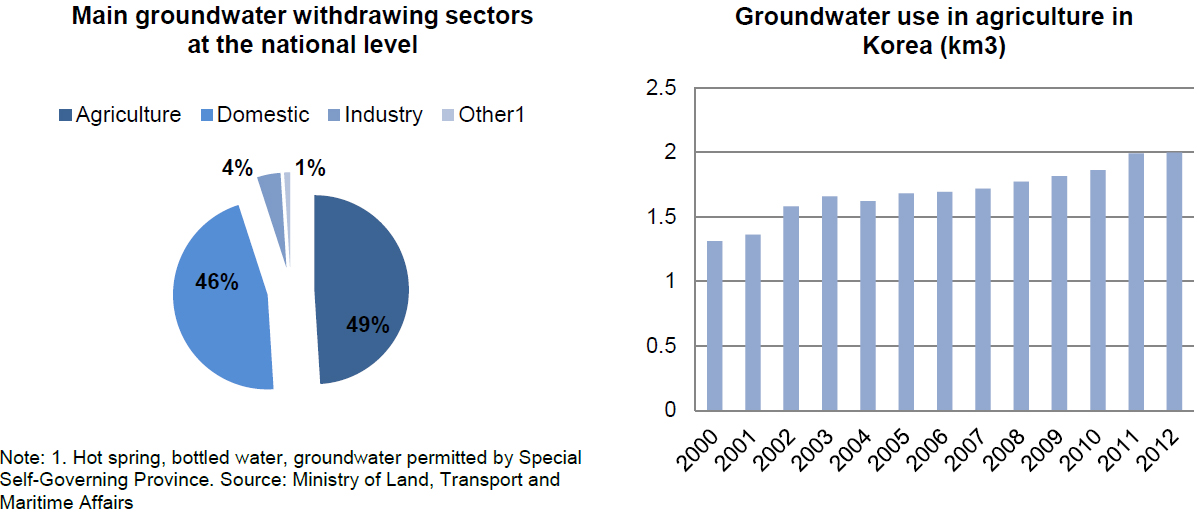
\includegraphics[width=\textwidth]{ROK_groundwater}
\end{figure}

\subsubsection{Climate Change, Forest Cover, and Hydrology}

As described earlier, \citet{nam2015has} found an increasing ET$_o$, which will reduce available water for plant growth and domestic use. 

\citet{Shin2014} modeled the effect of climate change on South Korea -- increasing temperatures and rainfall from current conditions to the 2080s. Using a modeled increase in temperatures and rainfall, they predicted potential forest cover changes and hydrology changes suggesting an increase in groundwater recharge. However, the ET increases XX\%, the forest cover will not change independent of leaf litter processes , soil-vegetation interactions, and species composition shifts. However, in spite of these uncertainties that with forest cover changes, stream-flow and groundwater recharge may not increase proportional to increases in precipitation in spite of a possible increase in precipitation. Thus, their results clearly demonstrate that our capacity to extend these models out (in this case 80 years) provides a planning horizon to that should be considered. 

\subsubsection{Hydrology and Food Linkages}

As noted earlier, water supply and food production, in particular rice production, is key for the Peninsula's food supply. In the next section, we will look more closely at the narratives with respect to food security and self-sufficiency and place these narratives into the water resources in terms of supply and quality.  

\section{Food and Water Linkages}

\subsection{Agriculture and the History of Irrigation}

Rice cultivation, as the major crop on the Korean Peninsula, was supported by a well developed irrigation system. For paddy rice, irrigation was indespensable practice and ancient Korea used a range of technologies that included construction of large-scale reserviors and conveyance systems. 

Managing water resources has been a documented endeavor in the Korean Peninsula for thousands of years. In fact, some of the earliest irrigation systems are well documented on the peninsula. The management of water and it's relationship to irrigated agriculture, especially paddy rice is well appreciated by the Koreans.

Agricultural activities started approximatly 8,0000 years ago. By the time bronze was introduced by the Huns, the agricultural life style was dominate for Koreans, who cultivated rice, barley, beans and among others. By the 4th century BCE, technology faciliated by the use of iron allowed the development of suctures such as Bo (weir) and Je-eon (reservoir) for crop irrigation.

Rice was the major crop cultivated in Korea from her ancient history. All irrigation water was primarily used in paddy fields for rice cultivation and only small portion of the water was used to partially irrigate upland cultivation.

According to ancient Korean history, irrigation of rice paddy was an indispensable practice. This is well shown by a large-scale reservoir, Byeokgol-je in Gimje, Jeonbuk province, which was built in 330 B.C. by King Biryu of Baekje Kingdom during the Three Kingdoms Era (Figure \ref{fig:Byeokgolje_embankment}). Although certinaly not the only one, structures such as this bare evidence the high level of Korean knowledge and techniques in building embankments.

\begin{figure}
\caption{Byeokgol-je Embankment (Source: \citet{TBD}.}
\label{fig:Byeokgolje_embankment}
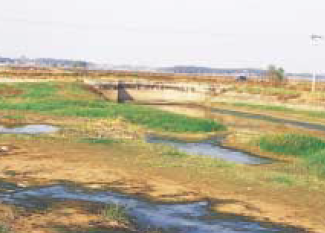
\includegraphics{Byeokgolje_embankment}
\end{figure}

However, it should be noted that technology was combined with strong centeralized government intent and political will to construct and restore irrigation facilities to increase farmland and production \citep{TBD}.

\subsection{Food (In)Security in Asia and Water}

North Korea is the outlier in East Asia with respect for food security. In the 1990s the North Korean economy saw stagnation turning into crisis. Economic assistance received from the USSR and China was an important factor of its economic growth. In 1991 USSR collapsed, withdrew its support and demanded payment in hard currency for imports. China stepped in to provide some assistance and supplied food and oil, most of it reportedly at concessionary prices.[citation needed] But in 1994 China reduced its exports to North Korea. 

Deprived of industrial inputs, including fertilizers, pesticides, and electricity for irrigation, agricultural output also started to decrease even before North Korea had a series of natural disasters in the mid-1990s. This evolution, combined with a series of natural disasters including record floods in 1995, caused one of the worst economic crises in North Korea's history. Other causes of this crisis were high defense spending (about 25\% of GDP) and bad governance. It is estimated \citep{TBD} that between 1992 and 1998 North Korea's economy contracted by 50\% and several hundred thousand (possibly up to 3 million) people died of starvation.

The rigidity in the political and economic systems of North Korea left the country ill-prepared for a changing world. The North Korean economy was undermined and its industrial output began to decline in 1990. From 1994 to 1998 North Korea suffered a famine. 

Since 1998 there has been a gradual recovery in agriculture production, which by 2013 brought North Korea back close to self-sufficiency in staple foods. However, as of 2013, most households have borderline or poor food consumption, and consumption of protein remains inadequate. Over 50\% of the population is food insecure (Figure~\ref{fig:foodinsecurity}). The situation is projected to improve only slightly by in the next 10 years with a decline from 53.8\% to 40.9\% of the population categorized as food insecure \citep{USDA2017projections}. 37\% of the children had their growth stunted and 1/3 of mothers were severely undernourished. 

\begin{figure}
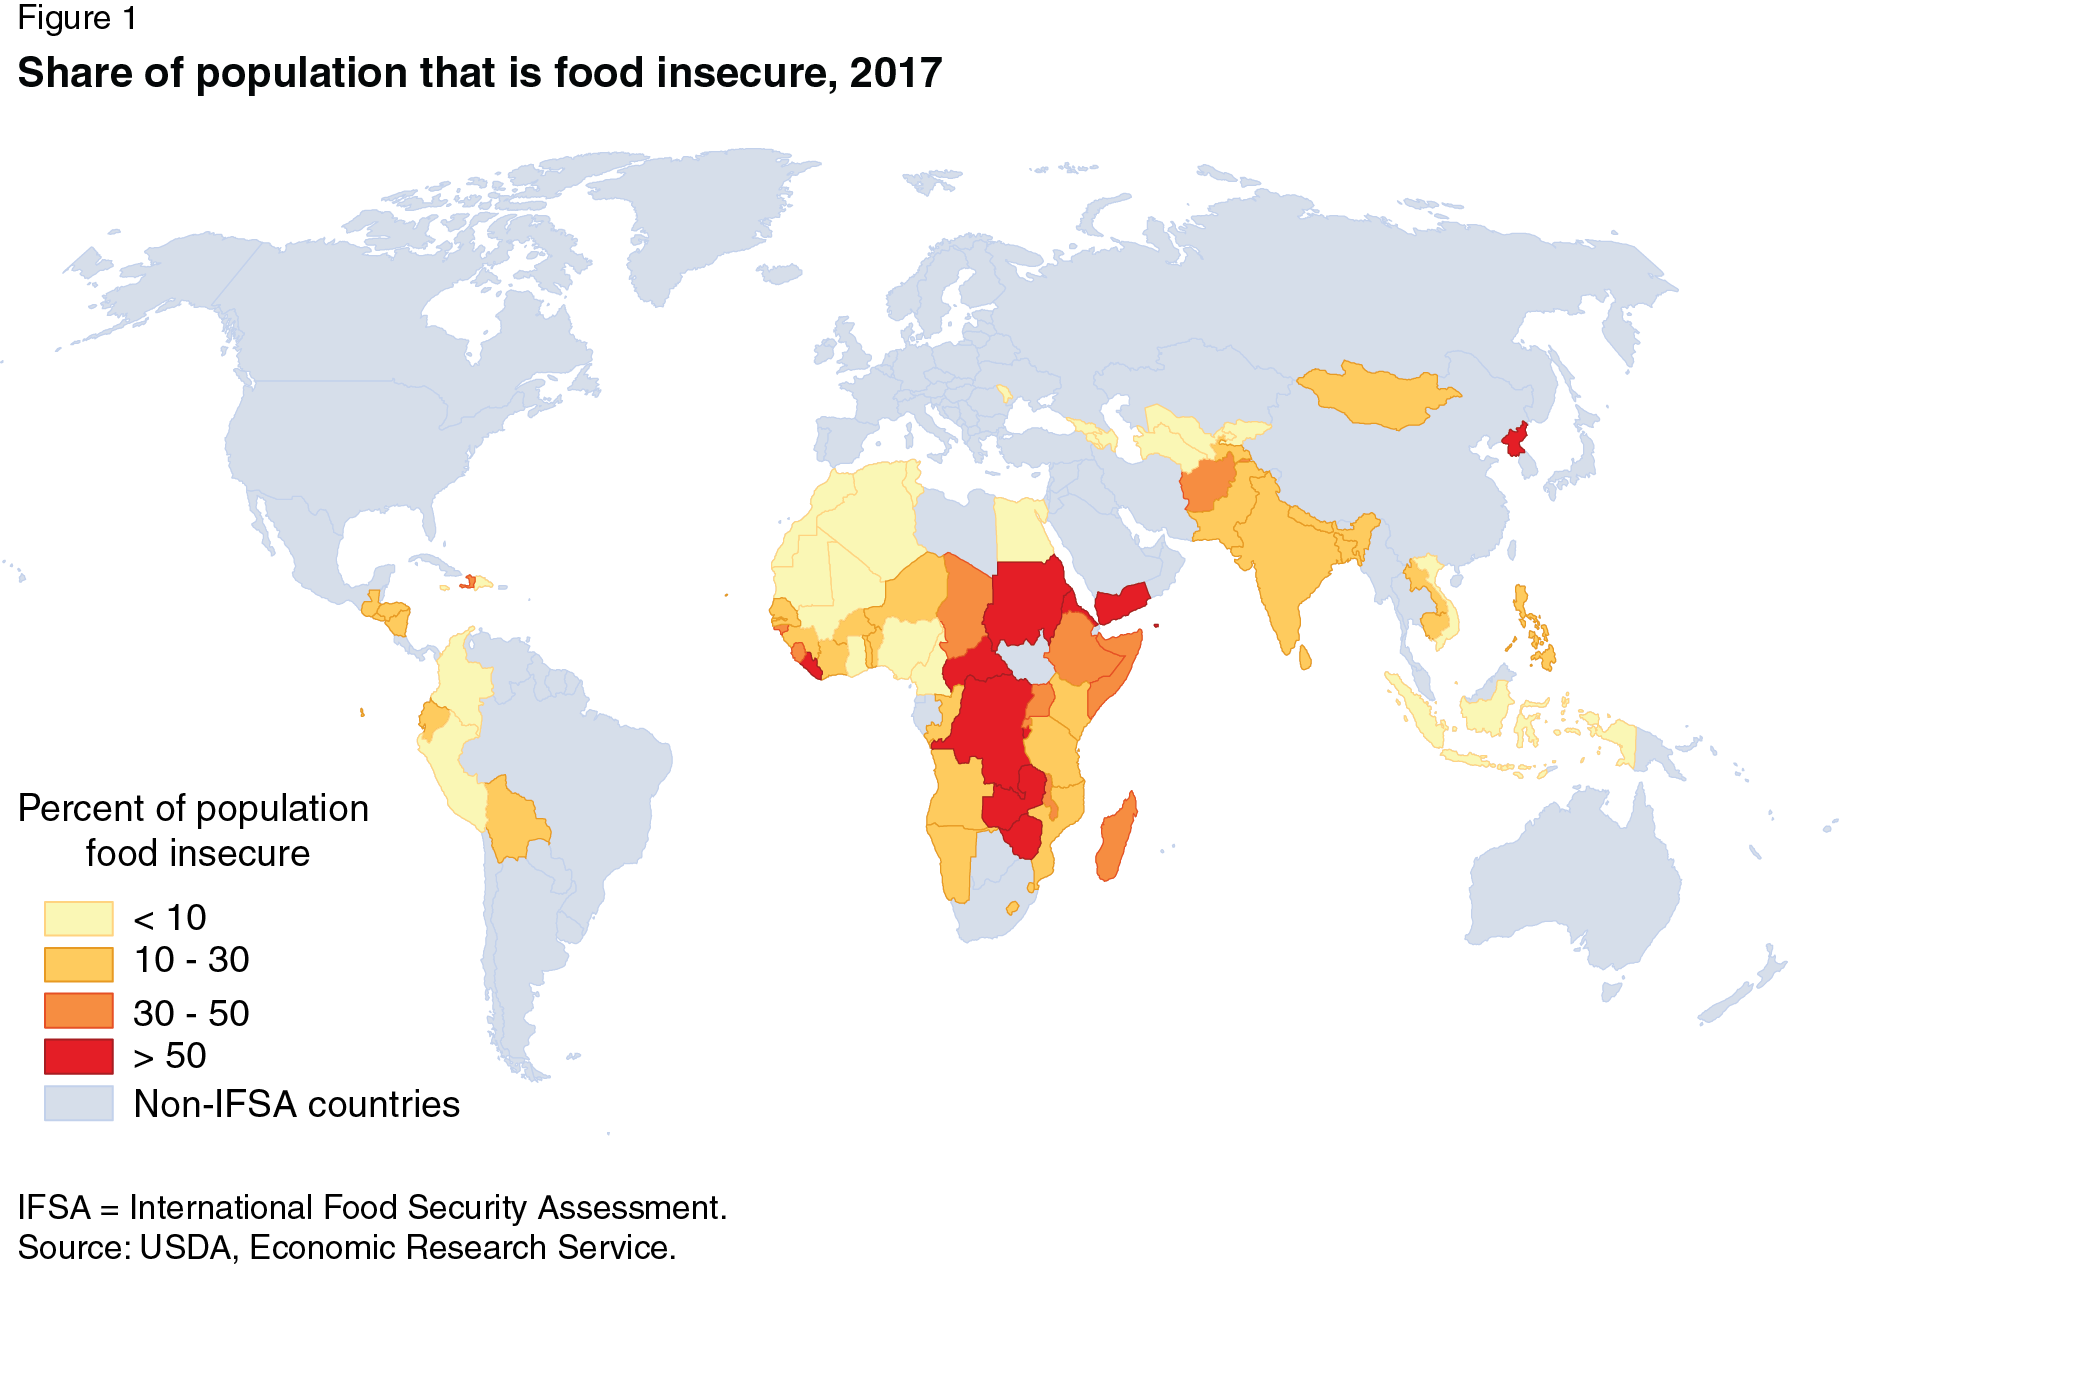
\includegraphics[width=\textwidth]{Food_Insecurity_World}
\label{fig:foodinsecurity}
\caption{Map of Worldwide Food Insecurity}  
\end{figure}

Meanwhile, few in South Korea regularly suffer from food shortages, while economic factors limit the protein content and dietary choices for a wide range of residents (IS this true? \citet{TBD}). 

While DPRK has historically depended on geopolitical allies for relieve during famine, without these partners the country's capacity to address famine is much more limit... MORE HERE \citet{rhie2017assessing}  According to the IFAD the decline of soil fertility in DPRKs contributed toe the lack of self-sufficiency in grad productions \citep{IFAD:1998}. 

Nevertheless, with the aid many claim that food does not reach the some of the most in need and may in fact re-enforce centralized power \citet{dalton2009feeding}. Nevertheless, informal markets began with aid and although gov't has been trying to limit the economic power of these markets with a range of tools, such as devaluation and creating a new currency. Of course, it's without any doubt that the aid was political, designed to promote a move away from totalitarian governance, thus entailed mixed motives. 

In summary, sustained massive government programs in the north have been used to address food security issues with limited success \citet{he2017there}. Meanwhile, as incomes have improved in the ROK, diets have changed and the capacity to develop food self-sufficiency has declined dramatically in the south. 

\subsection{Korean Diet}

According to \citet{kim2016korean}, the Korean diet is composed of bab and kuk and various banchan and Kimchi, which is both historically important and aesthetically \citet{chung2016aesthetics}. Overall, this diet includes a high proportion of vegetables, moderate to high consumption of legumes and fish, and low consumption of red meat \citep{kim2016korean}. However, to idealize the Korean diet fails to appreciate the long-term trend in both diet and the concomaninant impacts on environmental resources. 

\subsection{Westernizing Diets}

Over the long-term, the per capital supply of foods has dramatically changed. For example, barley as declined from 49 kg in 1960 to 1 kg in 2010, while rice has declined a bit and wheat has not no real change. Even more dramatic has been the increase in fruit ...

%(\Sexpr{round((46.2-6.6)/6.6*100, -1)}\%), eggs (\Sexpr{round((10.4-2.1)/2.1*100,-1)}\%), meat (\Sexpr{round((45.9-4.8)/4.8*100,-1)}\%), and milk (\Sexpr{round((54.9-0.2)/0.2*100,-3)}\%!) since 1960 \citep{Song:2017}. These changes have dramatic implications to water use and water quality --- although they may not impact the Korean Peninsula itself. 

\section{Water Resources, Infrastructure, and Management}

The management of water resources depends on judicious decision making based on the resources available. 

\citet{kim2018comparison}

Irrigated area relative to total paddy rice increased dramatically in Korea between 1918 and 1939 from 17\% to 70\% \citep{kikuchi1978agricultural}. The development of water, although with a long history in the Peninsula, rapidly changed in the early 20th Century with the colonial Japaneese along with the introduction of higher yielding Japanese varieties. 

The ROK invested heavily to improve agricultural productivity and even more so in the midde and late late 20th Century. According to \citet{burmeister1987south} the South Korean governement promoted an extremely directed research and extension to promote green revolution technologies. 

North Korea announced in December 1993 a 3-year transitional economic policy placing primary emphasis on agriculture, light industry, and foreign trade. A lack of fertilizer, natural disasters, and poor storage and transportation practices have left the country more than a million tons per year short of grain self-sufficiency. Moreover, lack of foreign exchange to purchase spare parts and oil for electricity generation left many factories idle.

The government pursued Kim Jong Il's Songun policy, under which the military is deployed to direct production and infrastructure projects. As a consequence of the government's policy of establishing economic self-sufficiency, the North Korean economy has become increasingly isolated from that of the rest of the world, and its industrial development and structure do not reflect its international competitiveness.

\subsection{Water Supply and Global Warming}

According to XXX, 

However, as several authors correctly point out, the impact of climate change provides imporant feedback on ecological and agroecological systems. For example, \citet{nam2015has} found a decline in ET$_o$ for many parts of South Korea...


\subsection{Surface-Ground Water Interactions}

South Korea lacks the awareness and interest in hyporheic zones, owing to which there are no management initiatives at all \citep{kim2018comparison}. Therefore, it is practically impossible to study this zone in Korea. During the period 2008--2012, the Ministry of Land invested US \$20 billion in the Four Major Rivers Project, focusing only on the functional aspects of water resources. The project focused on surface water, while ignoring groundwater and aquatic ecosystems. In addition, the proposal to change the designation of the five major river areas that the Ministry of Land has been promoting since 2013 was directly opposed to the conservation management plan for waterfront areas created by the Ministry of Environment.

Urban and rural landuse patterns have differential impacts on water quality. For example, in the City of Seoul, groundwater quality discharges into subway tunnels. Water quality in these tunnels has elevated Mn, Fe, NO3, and pathogenic microbe exceed Korean Drinking Water Standards \citep{chae2008hydrochemistry}. Of course, no one suggests that subway tunnel waters is a drinking water source, however, it demonstrates the connection (new connection) between subterrenan surface waters and ground water. 

\subsection{Water Quality: Nutrients and Drinking Water}

As one important component of the surface and ground water interactions is the contamiation of groundwater via reacharge that might enter groundwater via the hyperheic zone. In a study by \citet{min2003geologic}, shallow groundwater was contaminated... 

\begin{figure}
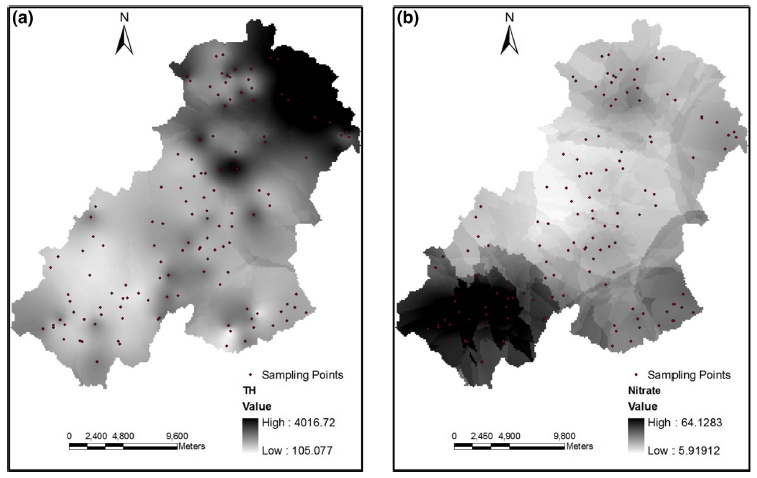
\includegraphics[width=\textwidth]{Tolera_groundwater}
\caption{ (Source: \citet{tolera2017spatial}). }
\label{fig:Tolera}
\end{figure}

In a country wide estimates, NK has an average N/ha use, while SK has an order[?] of magnitude more with XX N/ha. This is the difference between developed and ``developing'' countries. 

Given high levels in SK, we should expect elevated nutrients in surface and ground waters, which is highly spatially even. Nitrate is largely derived from chemical fertilizers with fractional contributions of 0.35-0.71, and organic fertilizers including composted manure with mixing fractions of 0.39-0.49 \citep{kim2015quantification}. 

Nitrogen and oxygen isotope have been used to evaluate the fate of nitrate in South Korea \citep{koh2010land} AND I CAN'T FIND THE TAKE HOME MESSAGE YET.

The relative contribution of nitrate from composted manure compared to chemical fertilizers increased with increasing nitrate concentrations, suggesting that composted manure significantly increases nitrate pollution and therefore its use should be carefully controlled to manage rural groundwater quality. This study also suggests that PCA and Bayesian isotope mixing models are effective for quantitative assessment of the sources of pollutants, such as nitrate. 

Nevertheless, for much of the country, the trend of declining groundwater contamination (Figure~\ref{fig:nitratechanges}) is a result of reduced nitrogen fertilizer inputs, which peaked in in 1990 at 1.104 Mt or 500 kg/ha \citep{lee2017unexpected}. In addition, throughout the 2000s the land areas dedicated toward agriculture has been declining and rice paddies having peaked in 1988 has been declining since.

\begin{figure}
\caption{Nitrate changes}
\label{fig:nitratechanges}
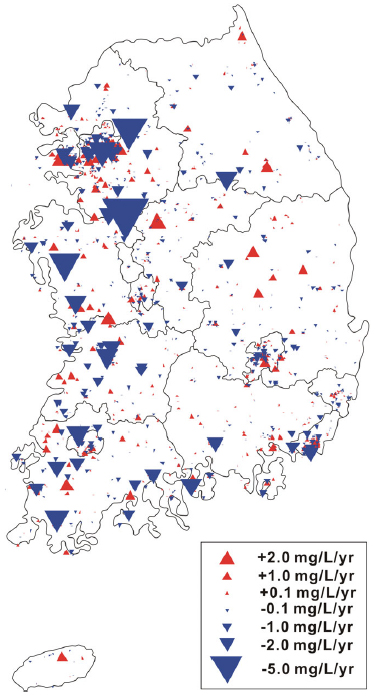
\includegraphics[width=\textwidth]{ROK_nitrate_changes}
\end{figure}

\subsection{Eutrophication: Inland Waters and Coastal Zone}

Natural lakes in South Korea are limited in number and generally quite small. As a result, reservoirs and regulated rivers are the major sources of freshwater for
society. About 18 000 reservoirs have been constructed in South Korea, and they are particularly important for domestic water supply. 

\citet{kim2001eutrophication} surveyed in this general assessment of the trophic state of South Korean reservoirs. Ten reservoirs were from the upper or middle reaches of rivers (including eight of the ten largest reservoirs in Korea), and three were estuarine reservoirs. Reservoirs in the mountainous district of South Korea were usually mesotrophic, whereas the estuarine reservoirs were highly eutrophic. Because total nitrogen to total phosphorus ratios were always between 18 and 163, phosphorus was probably more limiting than nitrogen for algal growth. However, hydraulic residence time and light penetration may be limiting in the nutrient-enriched downstream reservoirs. In winter, algal density was lowest in deep reservoirs, perhaps due to deep mixing. During the same season, algal density was high in shallow reservoirs, perhaps due to a favorable hydraulic residence time. Factors contributing to the observed eutrophication patterns, including nutrient runoff from agriculture, animal farms, fish aquaculture, and urban areas, are discussed. According to the national budget of phosphorus, fertilizer and livestock manure are major source of phosphorus, contributing 133400 and 73700 tons of phosphorus per year, respectively,
while human excretion discharges 30000 tons P/year. Reduction of the application of fertilizer, proper treatment of manure, and conservation of topsoil may be the most practical and effective measures to prevent further lake eutrophication.

Growing populations in northeast Asia have greatly altered the nitrogen cycle, with increases in agricultural production to feed the population, and with increases in N emissions and transboundary air pollution. For example, during the 1900's over 50\% of the N deposition over Republic of Korea was imported from abroad. In this paper, we present biogeochemical budgets of N for the South Korean peninsula (the Republic of Korea) and for the Yellow Sea region. We quantify N inputs from atmospheric deposition, fertilizers, biological fixation, and imports of food, feed, and products. We quantify outputs in riverine export, crop uptake, denitrification, volatilization, runoff, sedimentation and sea water exchange. Calculations were conducted using mean values from 1994--1997. All of the nitrogen budgets were positive, with N inputs exceeding outputs. The excess N inputs gave rise to increases in N storage in landfills and in groundwater. Annual accumulation of N in the Yellow sea, including inputs from South Korea and other drainage areas, was 1229 kt/yr with a residence time for N of approximately 1.5 years, thus doubling N content in marine waters every 3 years during 1994--1997 \citet{bashkin2002nitrogen}. The human derived N inputs leads to excessive eutrophication and pollution of the Yellow Sea.

\subsection{Water Quality and Pesticide Use}

TBD...

\subsection{Waste Water: Recycling and Treatment}

Climate change and the subsequent change in agricultural conditions increase the vulnerability of agricultural water use. Wastewater reuse is a common practice around the globe and is considered as an alternative water resource in a changing agricultural environment. Due to rapid urbanization, indirect wastewater reuse, which is the type of agricultural wastewater reuse that is predominantly practiced, will increase, and this can cause issues of unplanned reuse. Therefore, water quality standards are needed for the safe and sustainable practice of indirect wastewater reuse in agriculture. \citet{jeong2016irrigation} evaluated irrigation water quality criteria for wastewater reuse were discussed, and the standards and guidelines of various countries and organizations were reviewed to suggest preliminary standards for indirect wastewater reuse in South Korea. The proposed standards adopted a probabilistic consideration of practicality and classified the use of irrigation water into two categories: upland and rice paddy. The standards suggest guidelines for E. coli, electric conductivity (EC), turbidity, suspended solids (SS), biochemical oxygen demand (BOD), pH, odor, and trace elements. Through proposing the standards, this study attempts to combine features of both the conservative and liberal approaches, which in turn could suggest a new and sustainable practice of agricultural wastewater reuse.

In spite of the low temperature during the winter season and the high land environment, the wetland treatment system is gaining popularity in Korea because of its lower construction cost and simplicity in operation and maintenance. Many different types of wetland treatment systems have been built during the last 10 years, among which the free water surface wetland has been predominant. Most of the large-scale systems are government projects for improving the water quality of the streams flowing into the estuary dikes and reservoirs. The covering plants used in this system are different in different areas but cattails and reeds or their combinations are common. Constructed wetlands in Korea can be characterized by their shallow depths and short hydraulic residence times. There is no established flow pattern and configuration rules for constructing wetlands, but many efforts have been made with a view to improving their ecological function. Flow control is the most difficult problem in designing a riverbed or riparian wetland. There have been scores of flow rate control devices developed for wetlands, but none of them guarantee wetlands' safety against flooding. In earlier wetland construction, the building materials were mainly soil. Recently, strong and durable building materials such as rocks, gravel beds, concrete and steel are used at vulnerable places to protect them from erosion. \citet{youngchul2006experiences} investigation indicated that the wetland system would be an appropriate technology because it is not only cheaper to construct, but also requires less maintenance work. However, we suffer from the reduced effectiveness in performance during the winter. We need to evaluate the partial treatment accomplished during 6 to 7 months per year.


\section{Population and GHG Emissions}

\subsubsection{Declining Population Growth in the South}

The Korean Peninsula is home to 77 million people, about 2/3 are residents of South Koroea. But what's really striking is the speed at which it could happen: South Korea's population (currently larger than Spain) could shrink to a level comparable to tiny Switzerland within only a few generations. In 118 years South Korea is predicted to lose 40 million of its 50 million inhabitants, according to the research, which was conducted by a government agency. 

With no change in the growth rate, 1.19 children per woman, the southern portion of the pensula has begun experience a population decline (Figure~\ref{fig:popgrowth}), with a projected population of zero by the 2750 in 732 years, although these values were part of a study commissioned by the oposition party, South Koreans will probably experience the socio-economic impacts populations aging and deline.

Between 1975 and 2015, its median age soared to 41.2 from just 19.6. 

\begin{figure}
\label{fig:popgrowth}
\caption{Population growth in N and S Korea \citet{TBD}.}.
\end{figure}

And yet with a population density of as of 2017, 526/mile squared, while in the North \~210

\subsubsection{Korean GHG Production}

Greenhouse gas emissions have steadiliy increased in South Korea, and never passing the North's high in the 1990s (Figure~\ref{fig:carbonemissions}). However, more poignant is the precipitous decline in GHG emissions in North Korea. 

The decline is begins with collapse of the Soviet Union and then by the sanctions placed on the PDRK, who's residents are paying a severe price. Ironically, in terms of the GHG emissions, the country went from one of the worst per captia emitters in the 1990s to one of the lower countries. 

\begin{figure}
\caption{Korean Emissions (Source: \citet{TBD}.}
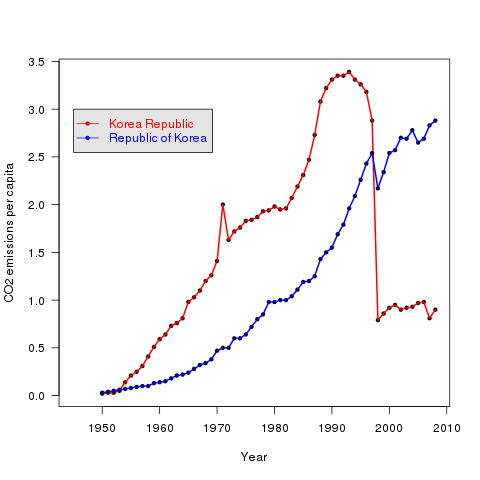
\includegraphics[width=\textwidth]{Korea_emissions}
\end{figure}



While the South Korean's emissions have stablized in recent years, relative to East Asian average (6.2 is still quite high). 

Meanwhile North Korean negoiators have ... \citet{habib10dprk}



\subsection{Forest Protection and Food Production}

DPRK dramatically increases deforestation in the 1990s, 

A large part of the emissions from deforestation and forest degradation has occurred in developing countries, where the share of deforestation-related greenhouse gas emissions has been estimated at around 25\% (Houghton, 2005)

\citet{tubiello2015contribution}

Major forest losses, of more than 0.5\% annually, have occurred in the tropical forests of West and East Africa, South and Central America, and Southeast Asia (FAO, 2008). However, there have been significant net forest gains in East Asia (3.8 M ha/year) and Europe (0.7 M ha/year). In spite of these changes, deforestation remains a concern in Asia, the most populous continent in the world (Zhao et al. 2006). 

This study presents results from an analysis of deforestation in the Democratic People's Republic of Korea.

Forest cover declined in Asia between 1990 and 2000 but increased later (FAO 2010). There is also substantial regional variability in the forest cover change in Asia. 

Forest cover continued to decrease in North Korea (Engler et al. 2014). Deforestation accelerated in North Korea during the 1990s compared to the preceding decade not only in terms of quantity but also in shape (Kang and Choi 2014). 

Deforestation in North Korea in recent decades has been receiving attention due to its relationship with the famine and floods its people suffered. Between 1995 and 1996, several floods damaged much of the land used for agriculture. It was estimated that 1.3 million hectares of agricultural land was damaged and lost due to inundation and sedimentation (IUFRO 2007). The debris left afterward in lower elevation zones made the land unusable for growing crops (Kim and Chi 1998). This is a partial cause of the famine that occurred in North Korea in the 1990s, resulting in more clear-cutting of forest to expand the agricultural land (IUFRO 2007).


\section{Food Sufficiency and Sovereignty and Water Security on the Korean Peninsula}

\subsection{Economic Transitions}

Just a few decades ago, South Korea was a poor, traumatized country sending its own low-skilled migrants out into the world as an economic lifeline. It should be a point of pride that the country's rapid development --- the so-called ``Miracle on the Han River''---has turned it into a magnet for Asian immigration. But the demographic changes are coming fast, too. ``The demand for foreign workers will only intensify,'' says Park from the International Organization for Migration, ``so South Korea better prepare itself.''

\subsection{SSR and Water Foot Prints}

\citet{yoo2016estimation} evaluated the water requirements if the ROK were to fulfill ROK's food self-sufficient goals. In the context of a meat diet, the per capita water requirements for productin and consumption would need from %\Sexpr{32474 + 14965} Mm3 (2006-2010) to \Sexpr{36175 + 17291} Mm3 by the year 2020 as \Sexpr{round((sum(36175, 17291, 32474, 14965)-sum(32474 + 14965))/sum(32474 + 14965)*100-100, 0)}\% increase. 

There are few examples of increasing water supply for agricutlural production by 12\% in a matter of a few years. So, one if forced to wonder how these policy goals actually translate to implemetation efforts and what is the actually intent behind such goals. [NOTE: Albert suggest that this might be an ``empty policy'' because of free trade agreements and their impact on domestic agricultural production. Need to follow up.]


\subsection{Organic and Sustainable Water in Korea}

The land area decidicated to certified organic agriculture has increased from 14.9 M ha to 37.2 M ha between 2000 and 2011 \citep{willer2014current}. In regions like the Hongdong District, in ROK, organic production is a rejection of modern Fordist agricultural models to maintain social cohesion while maintaining economic sustainability \citep{kim2015co, suh2015communitarian}

Depending on how organic agriculture is implememented, it may or may not improve the overall sustainability in agriculture. However, by avoiding certain chemicals and restricting the certain cultural practices, organic agriculture is the most well known farming alternative that may improve water quality in many parts of the world. 

Organic agriculture and traditional farming methods and foods could have a significant effect on the environmental resources used in the country. By focusing on non-dairy and red meat production, ROK could improve it's self-sufficency and maintain tradiational Korean diets.... more here, what about the impact of free trade?

\section{Energy Portfolio}

\subsection{Conflated Policy Goals: Renewable Energy and New Energy Sources}

\subsection{Industrial Ecology: The Ulsan Eco-Industrial Park}



\subsection{Ucity}

\url{https://www.youtube.com/watch?v=GAGbi1-DWQg}


\subsection{Shared Goals}


In this paper, I argue that the ROK and DPRK have shared challenges to the development of food security and maintain reliable water supplies. Although each country has radically different development patterns, by sharing the Peninsula, they may have common goals that could be better solved in a collaborative manner. 

I am a biogeochemist and have been working in farming communities in California for nearly 20 years. Negotiating the balance between maintaining an economically productive landscape while protecting and restoring the aquatic ecosystems has been the focal point of my research activities. Using this background to review the context of the Korean Peninsula is a challenge. 

My knowledge for the Korean Peninsula is colored by inequalities how North and South Korea institutions engage with both their natural resources and the outside scientific communities. Since I am not a scholar of Korean history, politics, or natural resources, my analysis and engagement with the literature is fraught with uncertainties and potential errors. I will rely on the audience to correct my failings and hope that I offend few with my conclusions. 

According to \citet{rhie2017assessing}, ``no matter what management reforms the North Korean regime implements, the country's economic system remains the intrinsic stumbling block.'' (p. 283).

Trade- and reform-centered strategies are likely to provide a sustainable solution to North Korea's problems. Because of North Korea�s lack of comparative advantage in the production of grains, the production-oriented strategy fails to attain the country's minimum human needs target.




%\bibliography{Korea_Ag,../references}